\section{Ablauf der Implementierung}
\subsection{Umsetzung Graph}
\begin{frame}
\begin{center}
\begin{footnotesize}
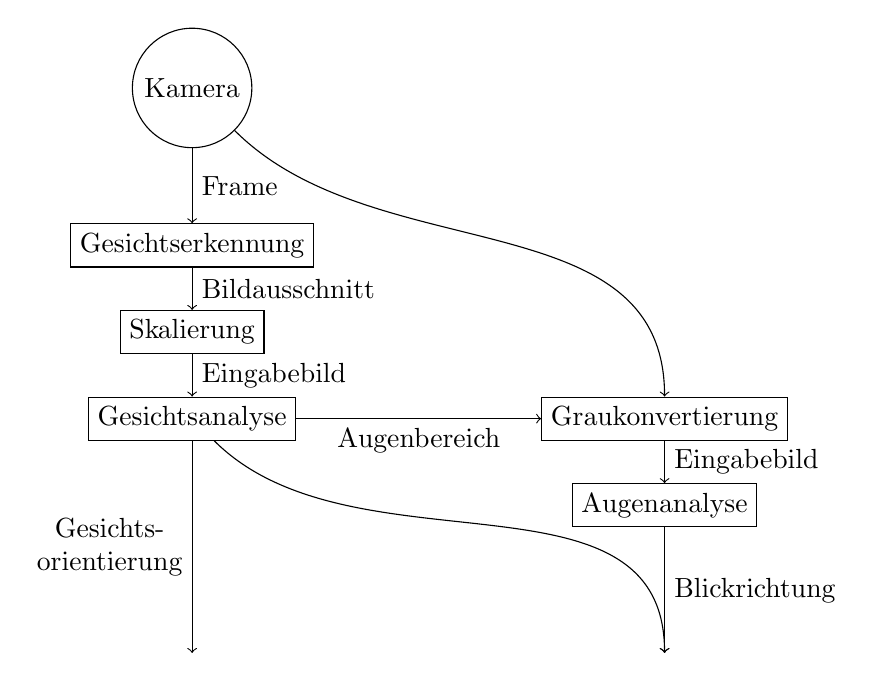
\begin{tikzpicture}
	\node[circle,draw,align=center] (C) at(0,0) {Kamera};
	\node[draw,align=center] (F) at(0,-2)  {Gesichtserkennung};
	\node[draw,align=center] (S) at(0,-3.1)  {Skalierung};
	\node[draw,align=center] (G) at(6,-4.2)  {Graukonvertierung};
	\node[draw,align=center] (A) at(0,-4.2)  {Gesichtsanalyse};
	\node[draw,align=center] (E) at(6,-5.3)  {Augenanalyse};
	
	\node (outA) at(0,-7.3)  {};
	\node (outB) at(6,-7.3)  {};
	
	\draw[->] (E)to node[right,align=center]{Blickrichtung}(outB);
	\draw[->] (A)to[out=-45,in=90] node[right]{}(outB);
	
	\draw[->] (C)to node[right]{Frame}(F);
	\draw[->] (F)to node[right]{Bildausschnitt}(S);
	\draw[->] (S)to node[right]{Eingabebild}(A);
	\draw[->] (A)to node[left,align=center]{Gesichts-\\orientierung}(outA);
	
	\draw[->] (A)to node[below]{Augenbereich}(G);
	\draw[->] (C)to[out=-45,in=90] node[left]{}(G);
	\draw[->] (G)to node[right]{Eingabebild}(E);
\end{tikzpicture}
\end{footnotesize}
\end{center}
\end{frame}
Da nur eine einzige fest montierte Kamera ohne Zoom eingesetzt wird, muss diese eine entsprechend hohe Auflösung besitzen, damit alle Personen zu erkennen sind. Zur Bestimmung der Blickrichtung sowie Kopfposition und Orientierung wird ein mehrstufiges Verfahren eingesetzt um alle Teilprobleme zu lösen.\\
Am Anfang müssen alle Gesichter, die im aktuellen Frame vorhanden sind, detektiert werden da nur auf diesen eine Berechnung ausgeführt wird.
Dabei machen die relevanten Bereiche nur einen sehr geringen Anteil des gesamten Bildes aus. Dazu wird die MTCNN Face Detection eingesetzt, siehe \autoref{MTCNN}, da dieses Verfahren im Vorabtests auf Probebildern einen sehr guten Eindruck gemacht hat und die meisten Gesichtern mit verschieden Größen und Blickrichtungen finden konnte. Laut Beschreibung des Verfahrens sollen sogar recht kleine Gesichter mit $20\times 20$ Pixeln erfassbar sein.\\
Für die weiteren Berechnungen muss bekannt sein, welcher Bereich von einem Gesicht im Frame eingenommen wird, um die relevanten Bildausschnitte aufzubereiten. Dabei muss das gesamte Gesicht in der Box sein, weitere Besonderheiten gibt es nicht, da OpenFace einen eigenen Facedetector besitzt. Je nach verwendetem Trainingsdatensatz und darin enthaltener Annotation werden z.B. Kinn und Haaransatz noch als Gesichtsbereich oder schon als außerhalb betrachtet. So geben beiden Methoden (OpenFace und MTCNN-Face) Boxen aus, diese sind in ihren Ausmaßen allerdings nicht identisch. Da die folgende Verarbeitung eine OpenFace-skalierte Box erwartet, hat sich eine Vergrößerung der Box um $30\%$ als sinnvoll erwiesen, bei Verwendung des MTCNN-Face Detektors um Ungenauigkeiten bezüglich der Position und Dimension des Kopfes im Bild entgegen zu wirken.\\
Sind mehrere Gesichter in mehreren Frames des Videos abgebildet, so muss auch eine Identitätszuordnung vorgenommen werden, damit bekannt ist welches Gesicht in Bild 1 welchem in Bild 2 entspricht. Für die Zuordnung reicht es meist aus, jene Box zu wählen, die am ehesten den selben Bildausschnitt repräsentiert wie im vorigen Frame. Dies ist ausreichend, da die Gesichter sich meist weder groß Bewegen noch sich die einzelnen Boxen der Probanden überlappen.\\
Damit sicher auf allen Gesichter gerechnet werden kann, ist eine semiautomatische Korrektur erforderlich um Falsch-Detektionen zu entfernen und fehlende Boxen der Gesichtern ergänzen zu können. Die gefundenen 5 Landmarks von MTCNN-Face Detection sind für die nachfolgende Berechnung nicht relevant, da sie gerade bei kleinen Gesichtern zu ungenau sind. Daher können alle bisher unternommenen Schritte auch von anderen Verfahren übernommen werden, da es sich hierbei nur um ein Vorverarbeitungsschritt handelt und zur Beschleunigung sowie Stabilität des späteren Berechnung beitragen soll.\\
Damit das Verfahren im nächsten Schritt zuverlässig arbeiten kann, werden alle zu kleinen Bildbereiche hochskaliert, um die Gesichter auf eine Mindestgröße zu bringen, siehe \autoref{scale_Algos}\\
Diese Bildbereiche werden nun von OpenFace weiterverarbeitet um die Landmarks, die signifikanten Punkte eines Gesichtes, zu bestimmen. Durch die vorige Zuordnung der Gesichert kann das Verfahren gezielt auf den Person arbeiten und entsprechend einstellte CLNF verwenden, um bessere Ergebnisse zu erzielen, siehe \autoref{OpenFace}. Außerdem könne alle gefundenen Personen gleichzeitig (parallel) ausgewertet werden.\\
Um die Position der Pupille noch exakter zu ermitteln wird ElSe verwendet, wozu eine Graukonvertierung durchgeführt werden muss, siehe \autoref{Graubild}. Ziel ist es, durch eine exakte Bestimmung der Pupillenposition, auch eine genaue Blickrichtungsbestimmung zu erhalten. Allerdings muss das Ergebnis von ElSe auf Plausibilität geprüft werden, um grobe Fehler zu vermeiden. Für die Umsetzung siehe \autoref{ElSe}.\\
Nun wird auf Basis der Landmarks und Kameraparameter die Position und Orientierung der Gesichter sowie die Blickrichtung bestimmt, siehe \autoref{calc_Position}. Diese Ergebnisse können dann von weiteren Anwendungen verwendet werden.